%%%%%%%%%%%%%%%%%%%%%%%%%%%%%%%%%%%%%%%%%%%%%%%%%%%%%%%%%%%
% --------------------------------------------------------
% Rho
% LaTeX Template
% Version 1.0 (28/04/2024)
%
% Author: 
% Guillermo Jimenez (memo.notess1@gmail.com)
% 
% License:
% Creative Commons CC BY 4.0
% --------------------------------------------------------
%%%%%%%%%%%%%%%%%%%%%%%%%%%%%%%%%%%%%%%%%%%%%%%%%%%%%%%%%%%
% --------------------------------------------------------
%					  FOR SPANISH BABEL
% --------------------------------------------------------
% \usepackage[spanish,es-nodecimaldot,es-noindentfirst]{babel}
% --------------------------------------------------------
%%%%%%%%%%%%%%%%%%%%%%%%%%%%%%%%%%%%%%%%%%%%%%%%%%%%%%%%%%%

\documentclass[9pt,a4paper,twoside]{rho}
\usepackage[english]{babel}
\usepackage{rhoenvs}

%----------------------------------------------------------
% TITLE
%----------------------------------------------------------

\title{ISO Day-Ahead Forecasting Using CNN-LSTM}

%----------------------------------------------------------
% AUTHORS AND AFFILIATIONS
%----------------------------------------------------------

\author[1]{Ali Camlibel}

%----------------------------------------------------------
% FOOTER INFORMATION
%----------------------------------------------------------

\etal{Camlibel et al.}
\footinfo{Creative Commons CC BY 4.0}
\smalltitle{\LaTeX\ Template}
\institution{The University of North Carolina at Charlotte}
\date{April 28, 2024} %\today

%----------------------------------------------------------
% ARTICLE INFORMATION
%----------------------------------------------------------

\corres{Provide the corresponding author information and publisher here.}
\email{example@organization.com.}
\doi{\url{https://www.doi.org/exampledoi/XXXXXXXXXX}}

\received{April 1, 2024}
\revised{April 3, 2024}
\accepted{April 20, 2024}
\published{April 28, 2024}

\license{Rho LaTeX Class \ccLogo\ This document is licensed under Creative Commons CC BY 4.0.}

%----------------------------------------------------------
% ABSTRACT
%----------------------------------------------------------

\begin{abstract}
    Independent System Operators (ISO) and Regional Transmission Organizations (RTO) are independent entities that ensure the reliability of the grid across the US. One way they do this is by facilitating the wholesale purchase and sale of power (MWh). Market participants bid to buy and sell power in real-time and in a day-ahead market. For the day-ahead market, bids and offers are entered in a day prior to the trading day. External factors can drastically affect load, and in turn, alter the price. To counter load change, intraday, real-time, trades must occur to keep the grid in balance. Often times, these contingency plans end up being more costly. Due to this price volatility, it is crucial for market participants to accurately forecast prices and hedge against this risk. This report aims to explore various deep neural network (DNN) architectures and proposes a configuration of convolutional neural network (CNN) and long short-term memory (LSTM) layers to forecast prices in different time windows.
    
\end{abstract}

%----------------------------------------------------------

\keywords{Keyword 1, Keyword 2, Keyword 3, Keyword 4, Keyword 5}

%----------------------------------------------------------

\begin{document}
	
\maketitle
\thispagestyle{firststyle}
% \tableofcontents

%----------------------------------------------------------

\section*{INTRODUCTION \& MOTIVATION}

Forecasting energy prices in the day-ahead market within ISO/RTOs is a topic of great interest to many market participant. Many different types of forecasting models have been used in the past, ranging from statistical models such autoregressive integrated moving averages (ARIMA) and support-vector machines (SVM) to artificial neural network based models such as recurrent neural networks and convolutional neural networks. ARIMA models can struggle against changing environmental conditions over a long period of time. For example, the increased generation of renewable generation. As solar generation replaces conventional coal and gas plants, the price of energy drops. Research has been done on this topic exploring various neural network architectures. The papers mentioned in this report specifically look at how artificial neural networks perform in this domain.

\section*{DATA COLLECTION}

Hourly price data was collected through the New-England ISO (NE-ISO) API (\url{https://webservices.iso-ne.com/docs/v1.1/}) from 2017 through 2024. Only a single locational marginal pricing (LMP) node - MASHPEE. 

\noindent The hourly weather data was sourced from the National Centers of Environmental Information's (NCEI) quality controlled datasets (\url{https://www.ncei.noaa.gov/access/crn/qcdatasets.html}). The weather features considered in this project are dry-bulb temperature, dew point, relative humidity, and cloud cover.

\section*{RELATED RESEARCH}

Deep learning for day-ahead electricity price forecasting (Chi Zhang, 2020) compared SVM and LSTM models for price forecasting. With the LSTM model proving better performance with an average mean absolute percentage error (MAPE) of 21.04\%. Price and weather data was incorporated, but additionally added prior load data (MWh), and gas prices (\$/MBTU). The basic principle of the model was to use a recurrent neural network with an LSTM cell unit to more effectively predict sequence data. The paper explored a similar time-horizon of predicting 24 hours ahead using 24 hours of prior data.

\noindent Figure 1 shows the hyper-parameters considered in this research's architecture.
\begin{figure}[H]
	\centering
	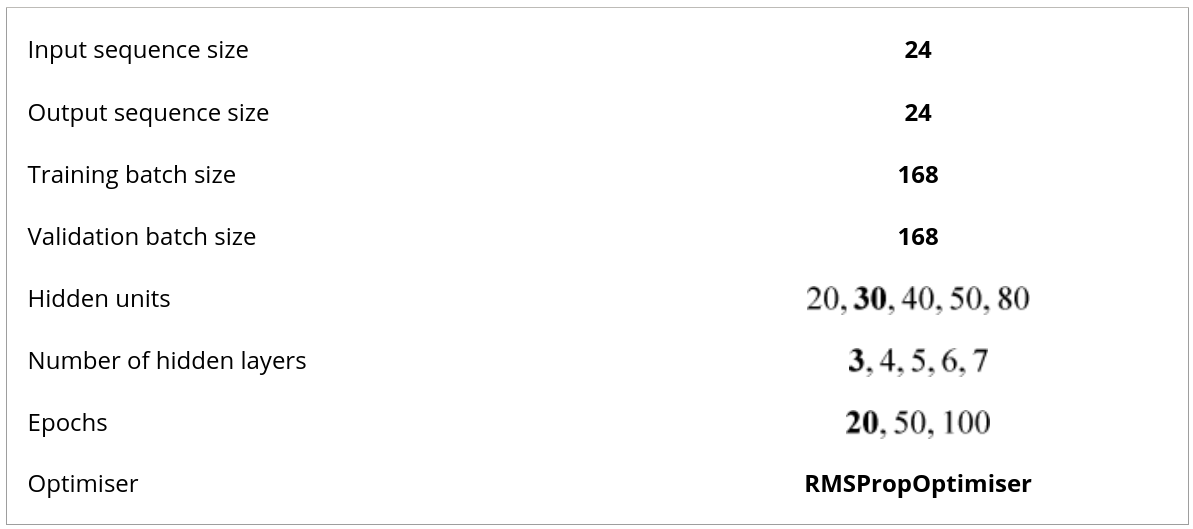
\includegraphics[width=0.8\columnwidth]{Figures/Research1.png}
\end{figure}

\noindent Power Market Price Forecasting via Deep Learning (Yongli Zhu, 2018) explored a LSTM architecture to predict prices. This paper also explored different forecasting windows such as 3, 6, 12, and 24 hours prior to predict the next hour. However, this model only explored 1 hour ahead pricing, and used a very small neural network consisting of 1 hidden layer with 4 LSTM cell units.

\vspace{-5em}

\section*{FEATURE ENGINEERING}

The hourly price data often follows a daily and yearly seasonality. Price tends to be higher during the summer and winter months due to cooling and heating requirements in households and businesses. Looking at the price curve for a given day, it generally follows a pattern where price is lowest in the middle of night and highest during the afternoon. The daily seasonality factors are due to residential, commercial, and industrial power demand.

\vspace{-4em}

\subsection*{Seasonality Figures}
Figure 2 shows yearly seasonality in the price data.
\begin{figure}[H]
	\centering
	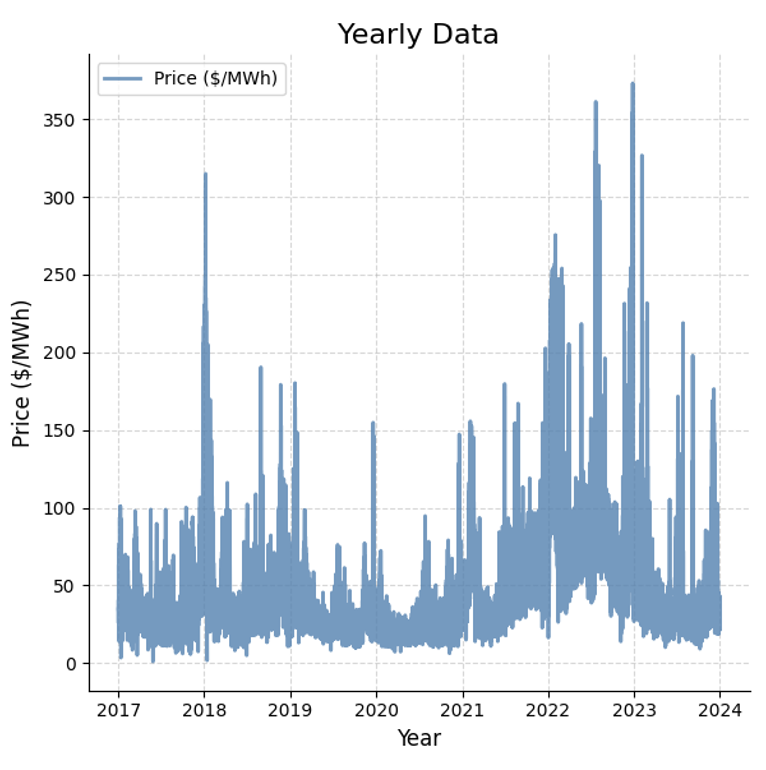
\includegraphics[width=0.8\columnwidth]{Figures/YearlySeasonality.png}
\end{figure}
            
Figure 3 shows daily seasonality in the price data.
\begin{figure}[H]
	\centering
	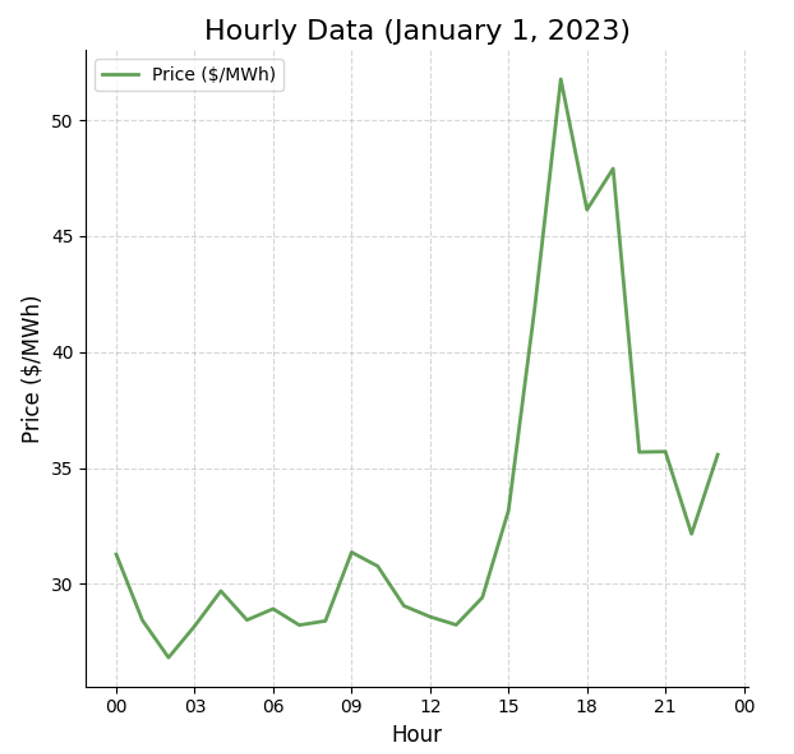
\includegraphics[width=0.8\columnwidth]{Figures/DailySeasonality.png}
\end{figure}
            
\noindent To capture this seasonality, feature engineering was performed to calculate sine and cosine values representing the instantaneous point the hour occurred.
    
\lstinputlisting[caption=Python code to calculate seasonality., language=Python]{seasonality.py}

\noindent Holidays were also considered. For each hour a binary field was set. This was done using the Python package \textit{holidays} (\url{https://pypi.org/project/holidays/}).

\section*{DATA PREPROCESSING}

For certain periods, prices could go up to \$500/MWh when on average it is \$20-\$100. Weather can also show dramatic peaks and dips due to inclement weather. Due to the non-stationary nature of price and weather, data was normalized before splitting and training. 

\noindent The min-max scaling technique was used, defined by the formula below.
\begin{equation} \label{eq:minmax_scaling}
	x_{\text{scaled}} = \frac{x - x_{\text{min}}}{x_{\text{max}} - x_{\text{min}}}
\end{equation}

\noindent The data contained 64,076 hourly observations. The first 60,000 observations were used for the training set, and the rest were used for testing. 10\% of the training set was used for model validation.

\section*{WINDOWING DATA}

The goal of windowing data is to turn a time-series problem into a supervised learning one. The data is shaped in such a way that each "window" is associated with one or more outputs. For example, the prior 24 time-steps of each step can be associated with 1 time-step into the future.

\noindent Figure 4 shows windowing 24 time-steps prior associated with 24 time-steps into the future.
\begin{figure}[H]
	\centering
	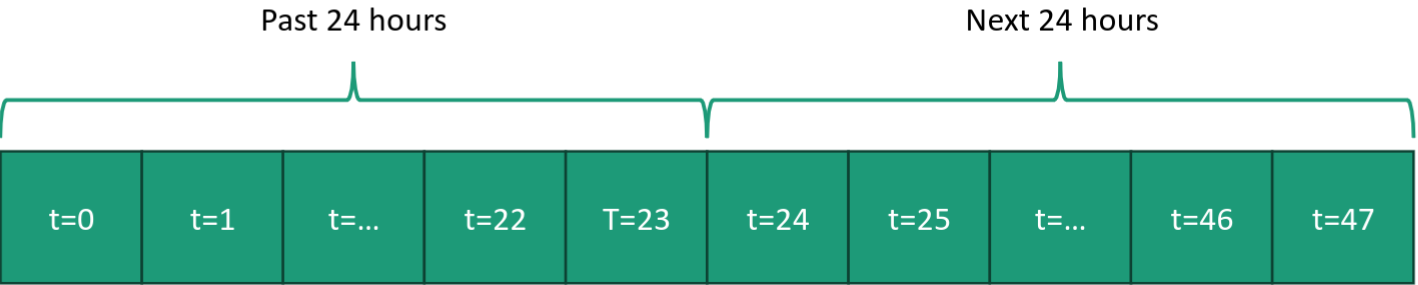
\includegraphics[width=0.8\columnwidth]{Figures/Windowing.png}
\end{figure}


\noindent The two window periods explored in this report are using 24 hours prior to predict the next hour and 24 hours prior to predict the next 24 hours. The code below ensures that there is enough of a window to get the start and end of the training and testing datasets by subtracting the number of past observations from the length and adding the number of future steps to the current index.

\noindent The function to window the data is defined below.
\lstinputlisting[caption=Python code to window data., language=Python]{window-data.py}

\section*{SARIMA ARCHITECTURE}

The first model was a simple univariate ARIMA model. Training the model was very intensive on CPU and took an extensive amount of time to train on the 7 years of price data. Only price was considered for this model. The main parameters of the SARIMA model (p, d, q) (P,D,Q) were set as (2, 0, 1) (2, 0, 1), using 2 lagged variables, no differencing, and 1 moving average term. The model ended up performing poorly, but proves that price does have temporal dependencies that can be learned.

\noindent Figure 5 shows the results of the SARIMA model for one week.
\begin{figure}[H]
	\centering
	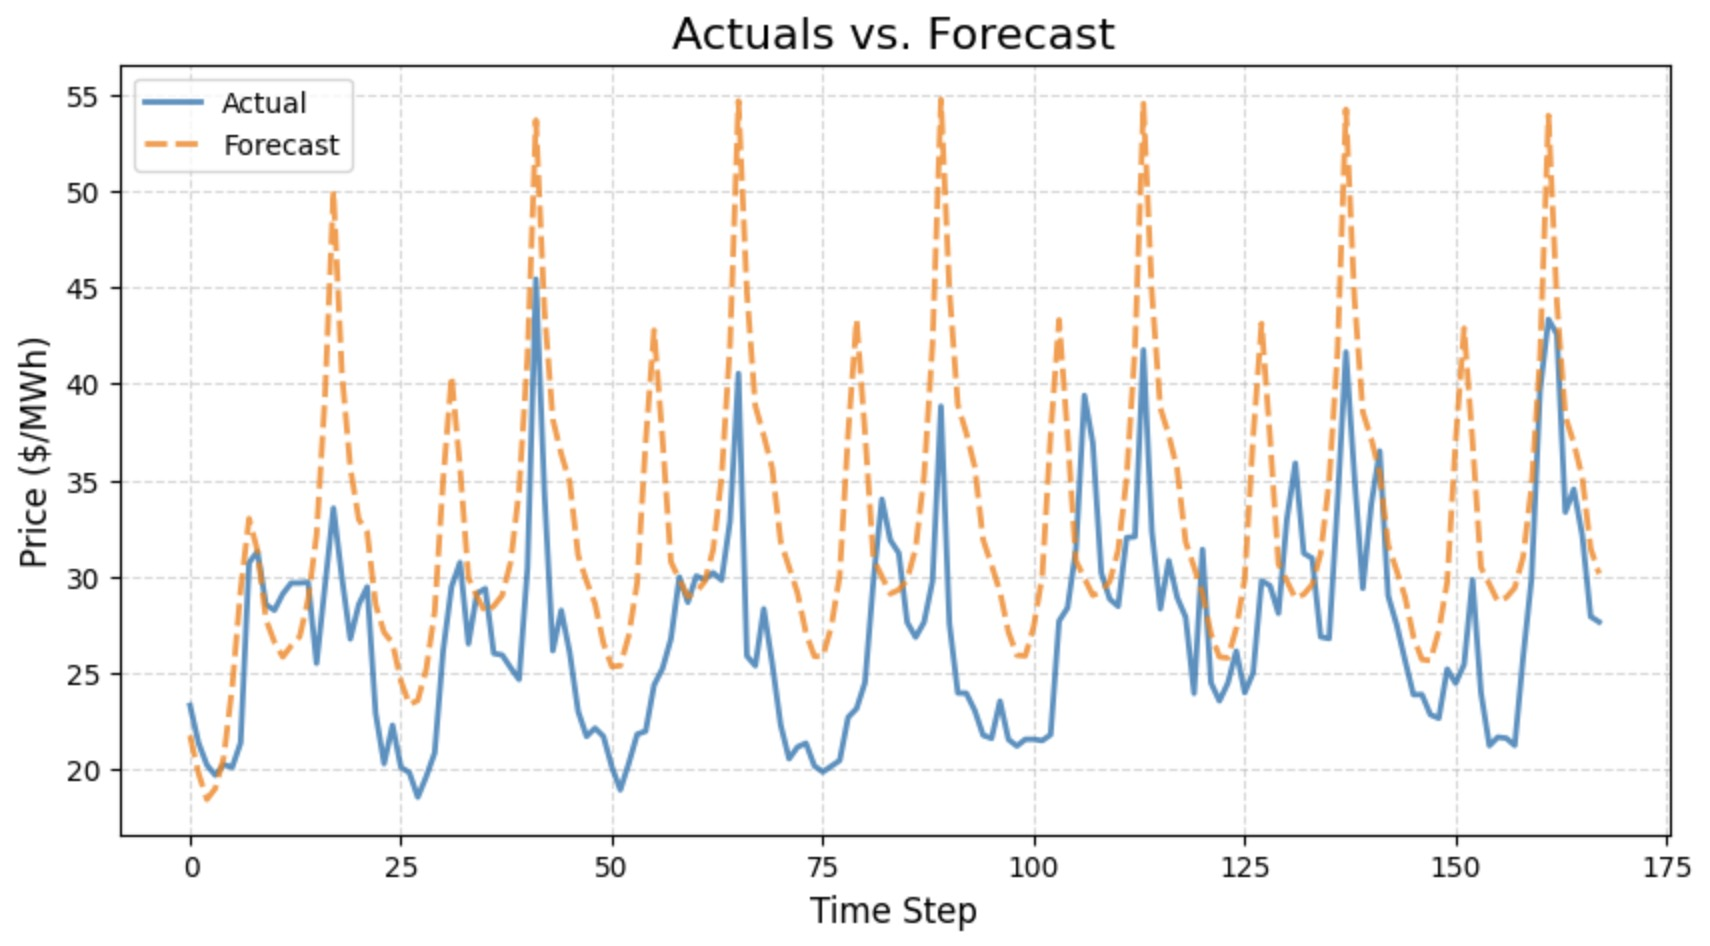
\includegraphics[width=0.8\columnwidth]{Figures/ARIMA_Results.png}
\end{figure}


\section*{DENSE LAYER ARCHITECTURE}

The first attempt at using neural networks was to build a simple feed-forward neural network with Dense layers.

\noindent Figure 6 shows the dense model architecture.
\begin{figure}[H]
	\centering
	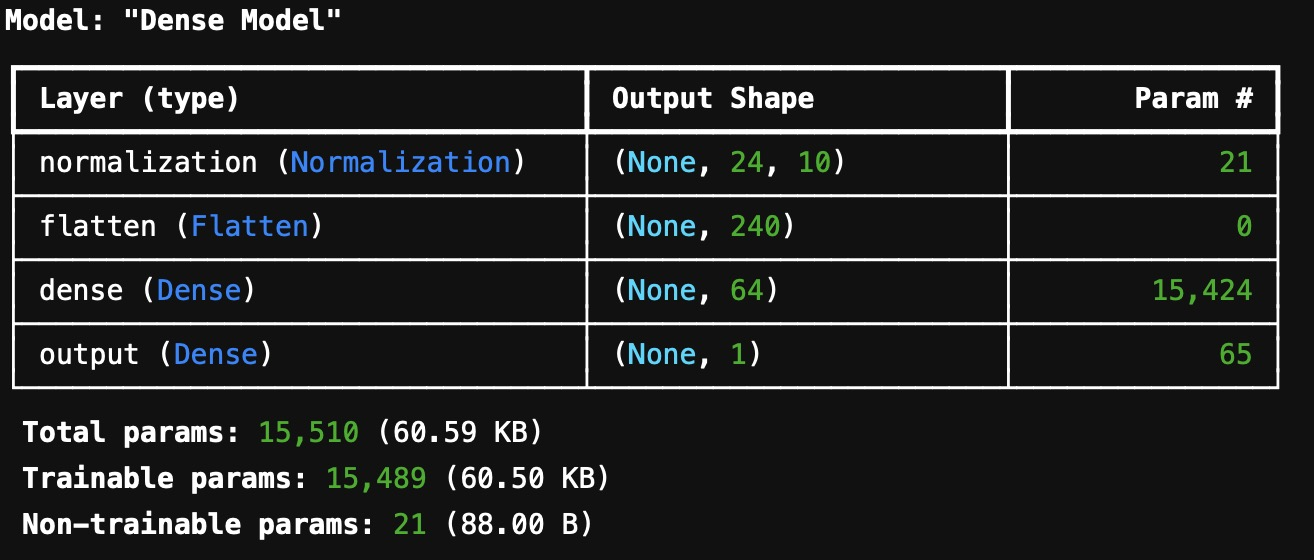
\includegraphics[width=0.8\columnwidth]{Figures/Dense_Architecture.png}
\end{figure}

\noindent Hyperparameters:
\begin{itemize}
	\item Neurons: 64
	\item Activation: ReLU
	\item Epochs: 100 /w EarlyStopping (patience=4)
	\item Optimizer: RMSProp
	\item Loss Function: RMSE
	\item Batch Size: 168
\end{itemize}

Two separate models were trained with this architecture. One for 24 hours prior to predict the next hour, and the other using 24 hours prior to predict the next 24 hours.

\subsection*{24 hours prior to predict 1 hour ahead}

\noindent Figure 7 shows the loss curve during training (24 hours prior, 1 hour ahead).
\begin{figure}[H]
	\centering
	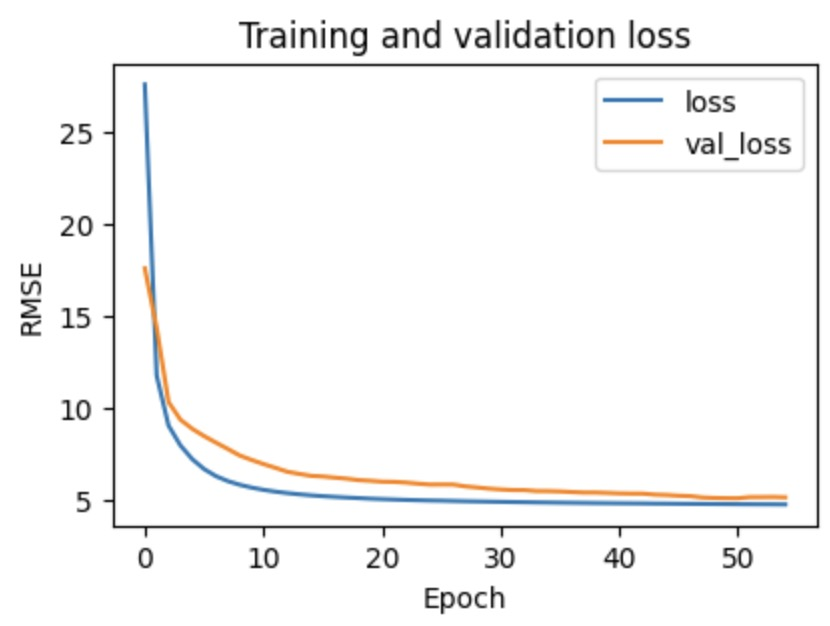
\includegraphics[width=0.8\columnwidth]{Figures/Dense_24_1_Learning.png}
\end{figure}

\noindent Over the test dataset, an average MAPE of \textbf{9.78\%}.\\

\noindent Figure 8 shows the results of forecasting 1 week.
\begin{figure}[H]
	\centering
	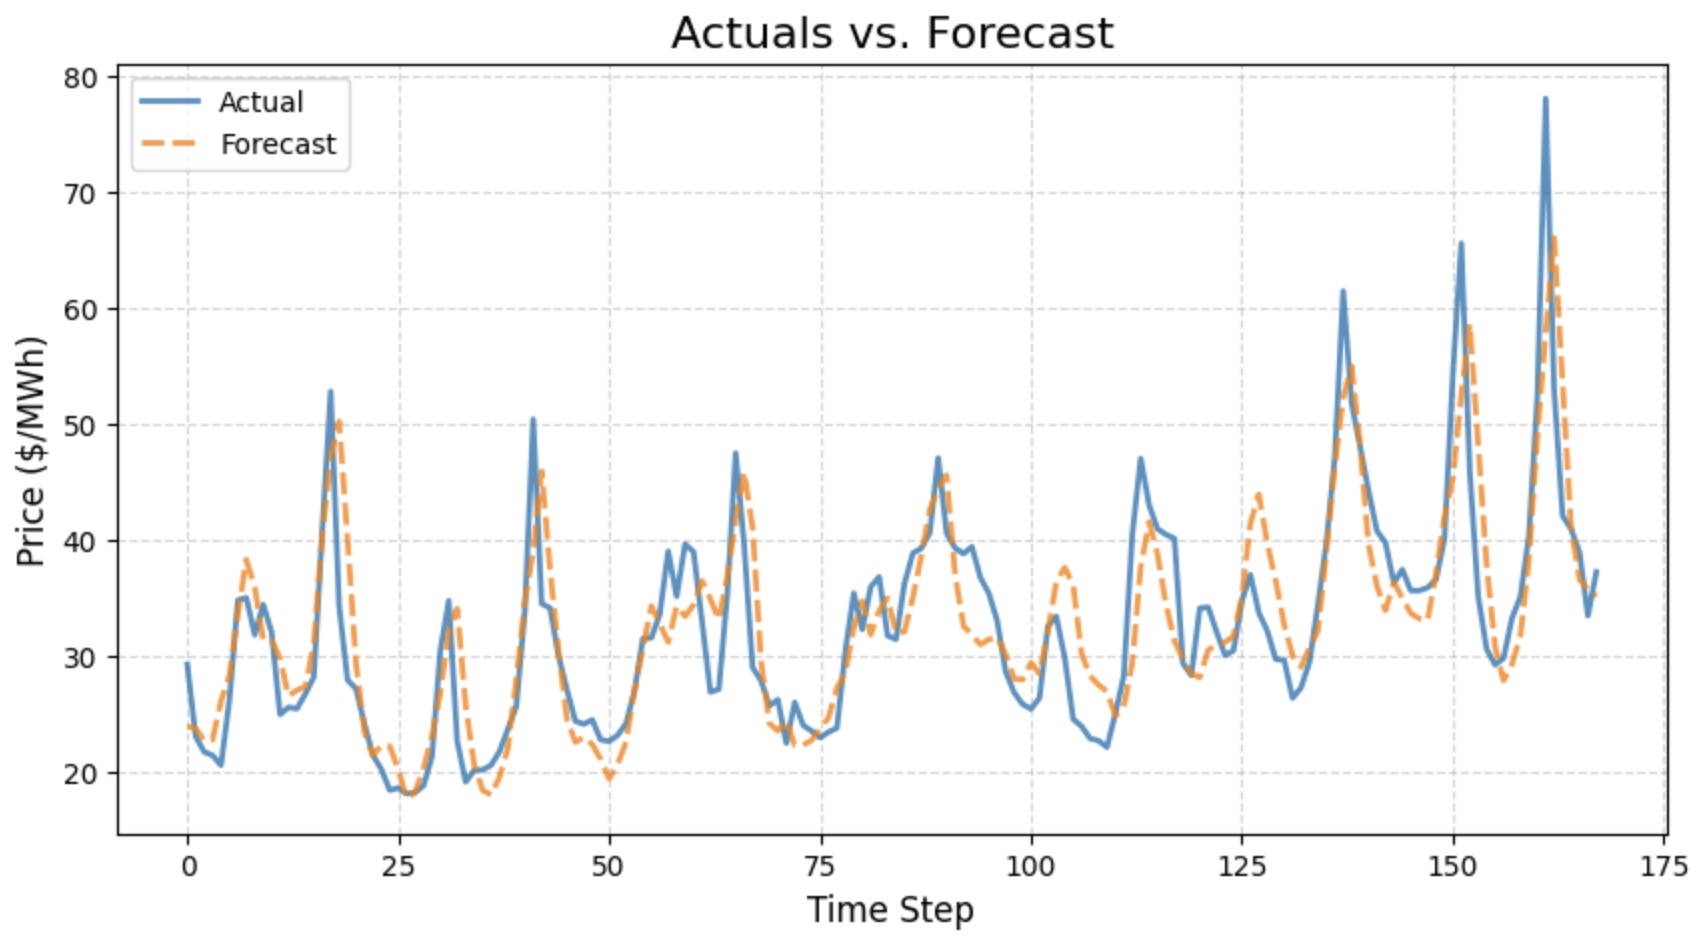
\includegraphics[width=0.8\columnwidth]{Figures/Dense_24_1_Results.png}
\end{figure}

\subsection*{24 hours prior to predict 24 hours ahead}

\noindent Figure 9 shows the loss curve during training (24 hours prior, 24 hours ahead).
\begin{figure}[H]
	\centering
	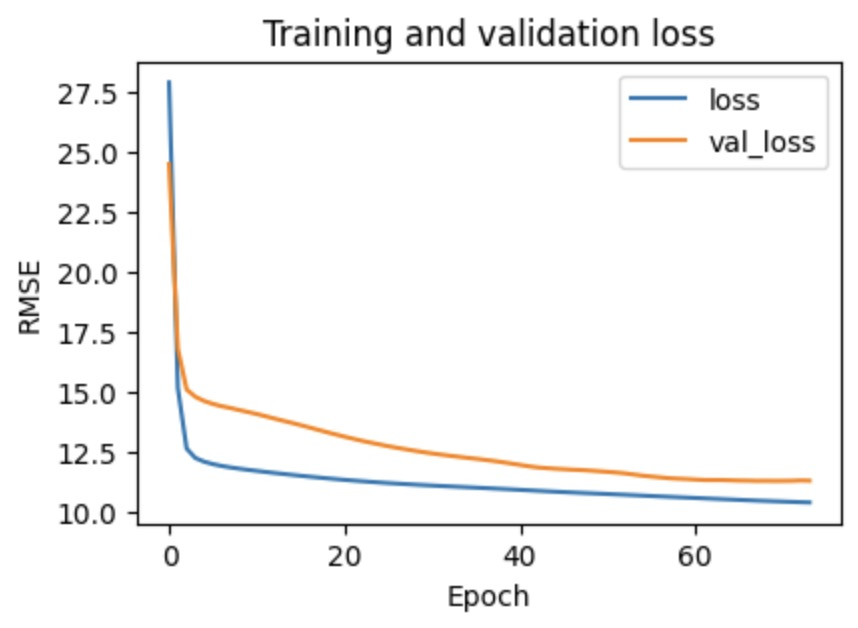
\includegraphics[width=0.8\columnwidth]{Figures/Dense_24_24_Learning.png}
\end{figure}

\noindent Over the test dataset, an average MAPE of \textbf{22.73\%}.\\

\noindent Figure 10 shows the results of forecasting 1 week.
\begin{figure}[H]
	\centering
	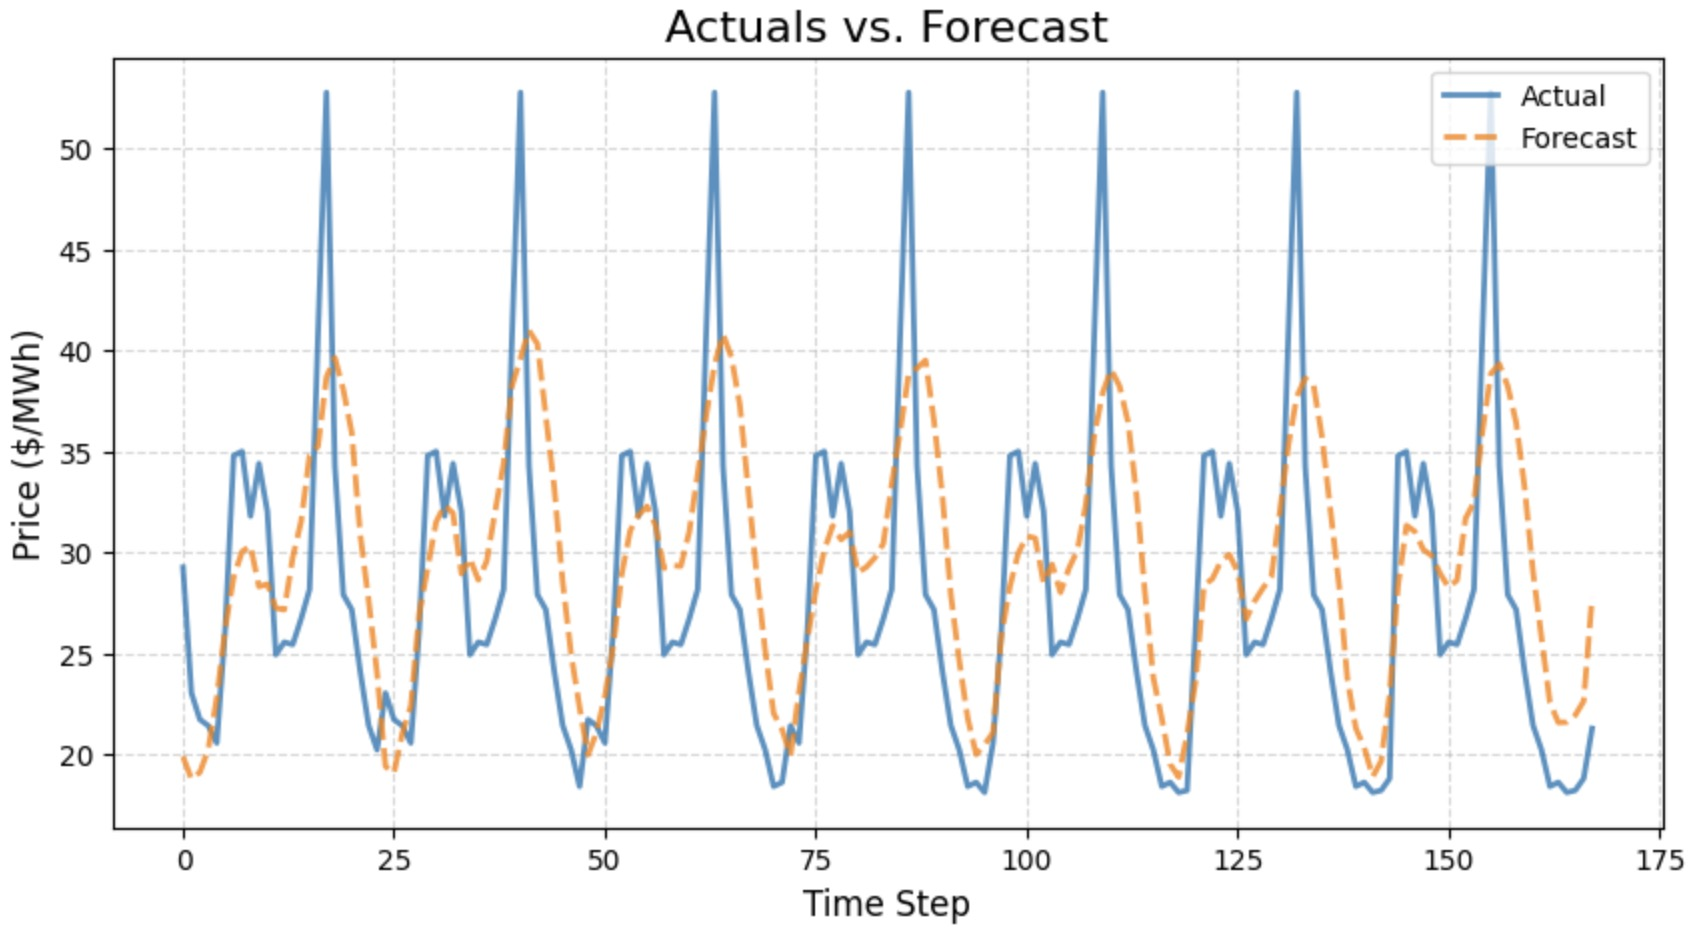
\includegraphics[width=0.8\columnwidth]{Figures/Dense_24_24_Results.png}
\end{figure}

\noindent This model performs poorly while predicting 24 hours ahead as it struggles to learn the peaks of each day, but it still seems like it's learning something. The supervised learning approach with the windowing function seems to work even on a Dense architecture.


\section*{CNN ARCHITECTURE}

A CNN architecture which uses a 1-d convolutional layer and max pooling was also considered. The idea behind using CNN for forecasting would be to better learn the inner relationships between the weather and seasonality inputs when it comes to price.

\noindent The input and output layers are similar to the dense architecture. Flatten is used after the max pooling layer to reduce the data to a single dimension, so that the dense layer can learn easier.

\noindent Figure 11 shows the CNN architecture.
\begin{figure}[H]
	\centering
	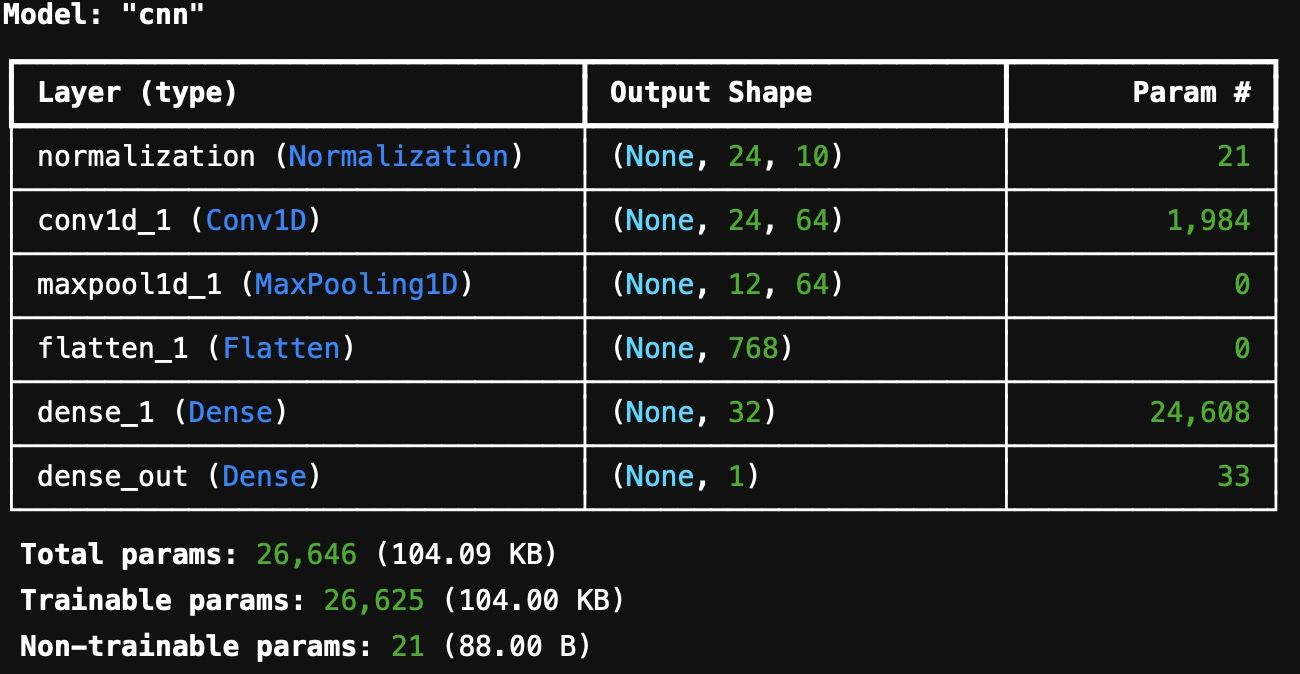
\includegraphics[width=0.8\columnwidth]{Figures/CNN_Architecture.png}
\end{figure}

\noindent Hyperparameters:
\begin{itemize}
	\item Filters: 128
	\item Activation: ReLU
	\item Epochs: 100 /w EarlyStopping (patience=4)
	\item Optimizer: RMSProp
	\item Loss Function: RMSE
	\item Batch Size: 168
	\item Kernel Size: 3x3
	\item Strides: 2
	\item Padding: same
\end{itemize}


\subsection*{24 hours prior to predict 1 hour ahead}

\noindent Figure 12 shows the loss curve of training.
\begin{figure}[H]
	\centering
	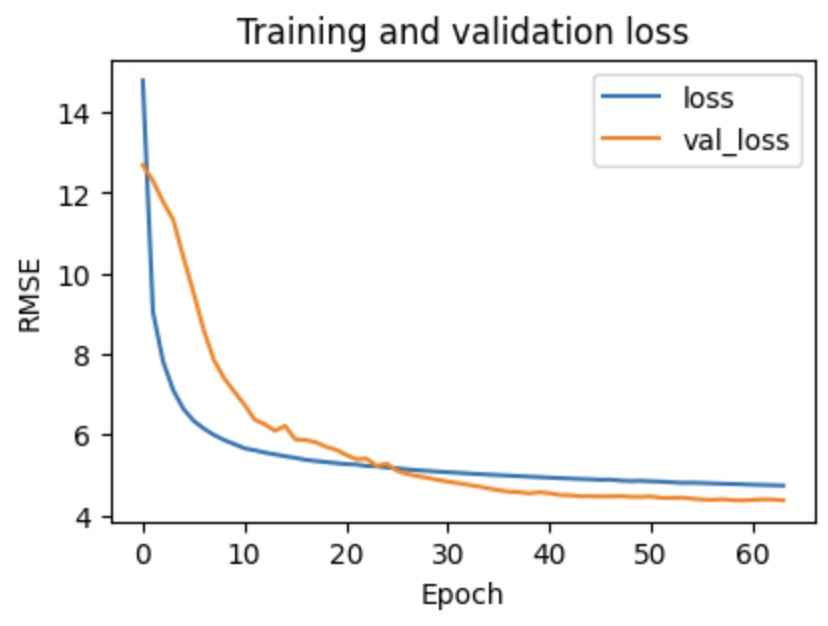
\includegraphics[width=0.8\columnwidth]{Figures/CNN_24_1_Learning.png}
\end{figure}

\noindent Over the test dataset, an average MAPE of \textbf{11.13\%}.\\

\noindent Figure 13 shows the results of forecasting a week.
\begin{figure}[H]
	\centering
	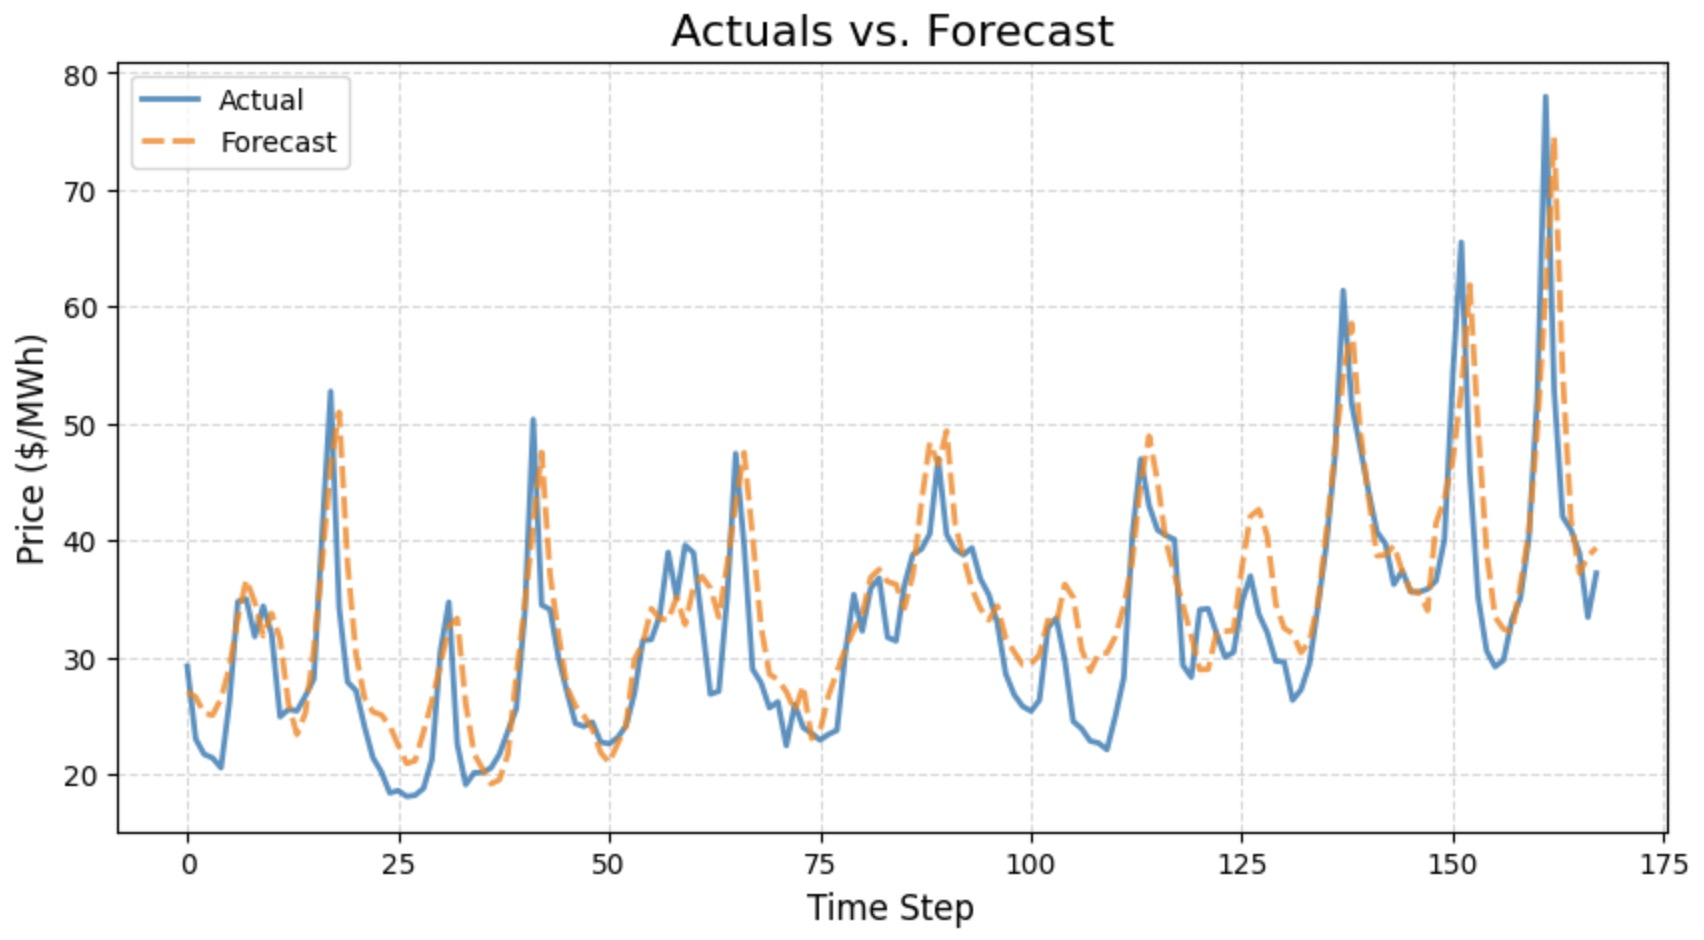
\includegraphics[width=0.8\columnwidth]{Figures/CNN_24_1_Results.png}
\end{figure}

\subsection*{24 hours prior to predict 24 hours ahead}

\noindent Figure 14 shows the loss curve of training.
\begin{figure}[H]
	\centering
	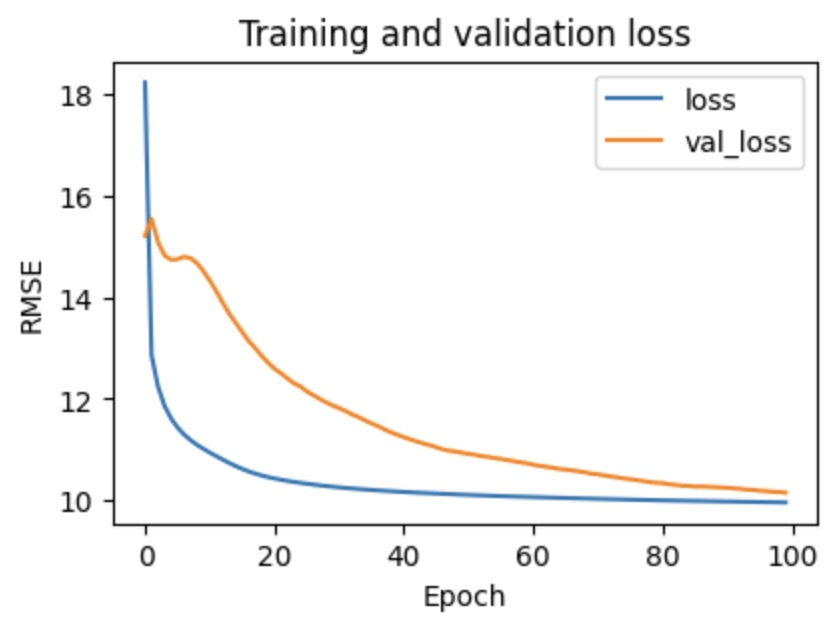
\includegraphics[width=0.8\columnwidth]{Figures/CNN_24_24_Learning.png}
\end{figure}

\noindent Over the test dataset, an average MAPE of \textbf{22.88\%}.\\

\noindent Figure 15 shows the results of forecasting a week.
\begin{figure}[H]
	\centering
	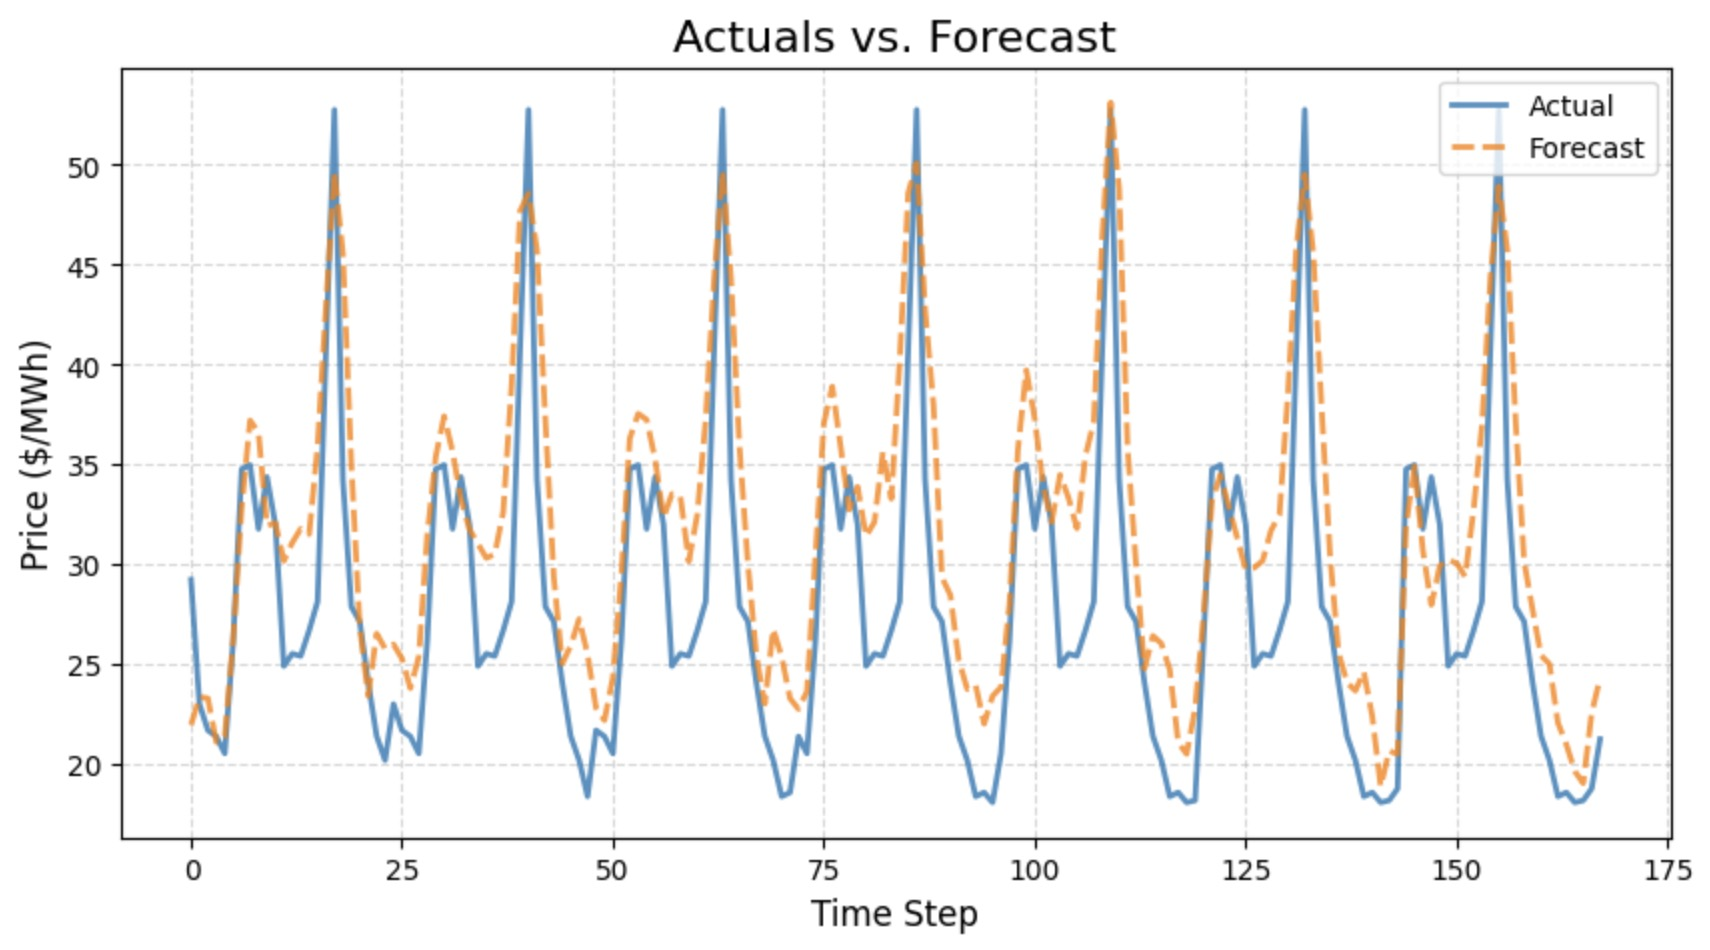
\includegraphics[width=0.8\columnwidth]{Figures/CNN_24_24_Results.png}
\end{figure}

\noindent Both CNN models seem to be similar to the Dense output, yet the 24 hour-ahead CNN model seems to better capture the peaks of each day compared to the respective dense model.

\section*{LSTM ARCHITECTURE}

The research in this report was primarily based on using recurrent neural networks (RNN) with LSTM cells to better forecast as there are temporal/sequential dependencies between the price and weather data.

\noindent Figure 16 shows the LSTM architecture.
\begin{figure}[H]
	\centering
	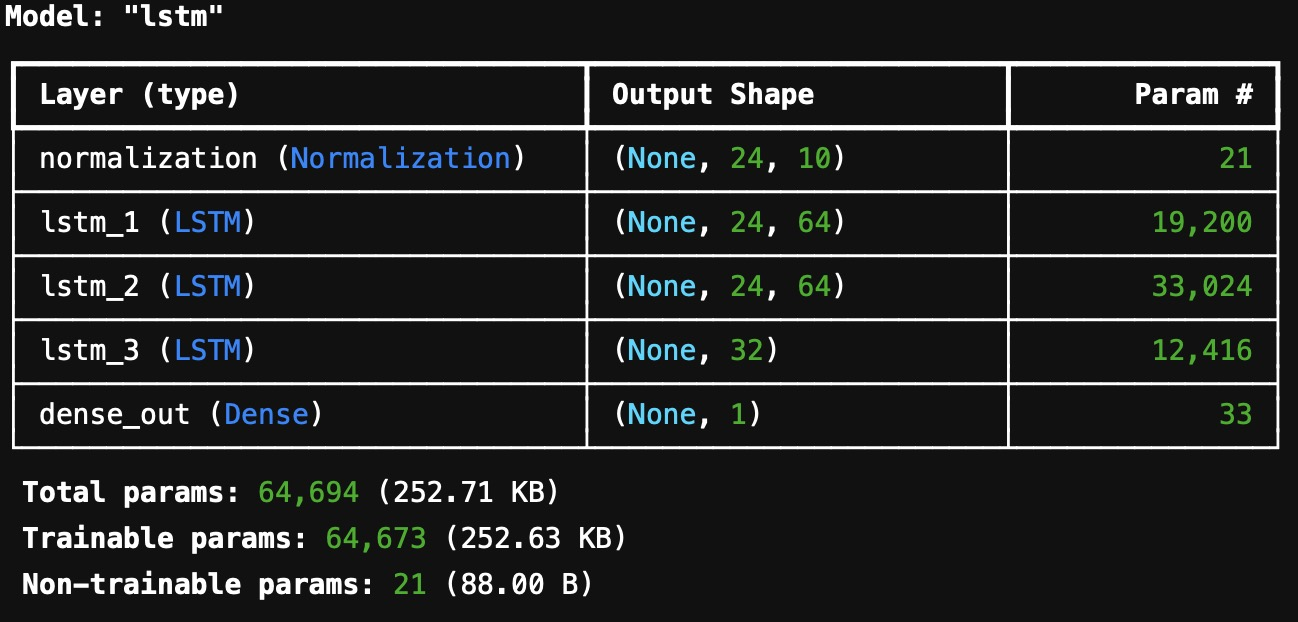
\includegraphics[width=0.8\columnwidth]{Figures/LSTM_Architecture.png}
\end{figure}

\noindent Hyperparameters:
\begin{itemize}
	\item Activation: ReLU
	\item Epochs: 100 /w EarlyStopping (patience=4)
	\item Optimizer: RMSProp
	\item LSTM cell units: 30
	\item Loss Function: RMSE
	\item Batch Size: 168
\end{itemize}

\subsection*{24 hours prior to predict 1 hour ahead}

\noindent Figure 17 shows the loss curve.
\begin{figure}[H]
	\centering
	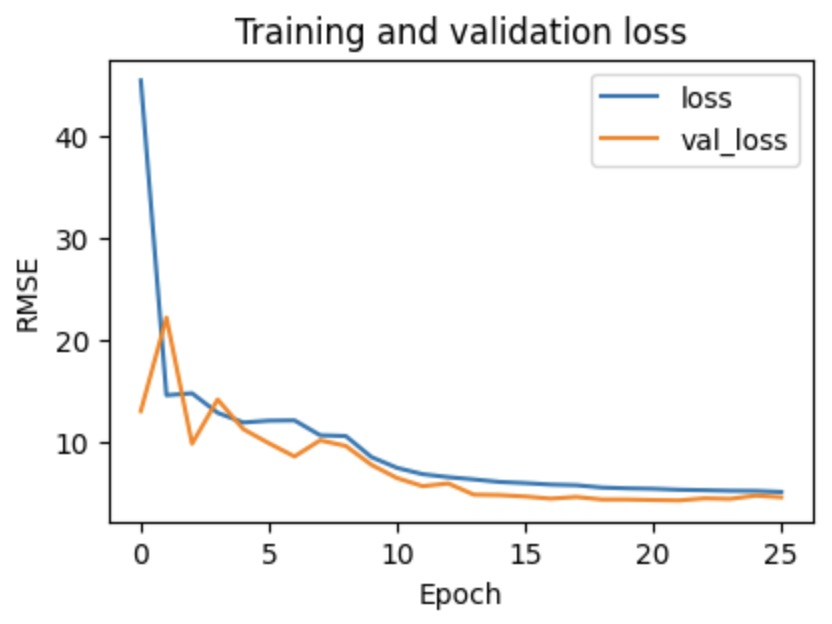
\includegraphics[width=0.8\columnwidth]{Figures/LSTM_24_1_Learning.png}
\end{figure}

\noindent Over the test dataset, an average MAPE of \textbf{10.66\%}.\\

\noindent Figure 18 shows the forecasting results for 1 week.
\begin{figure}[H]
	\centering
	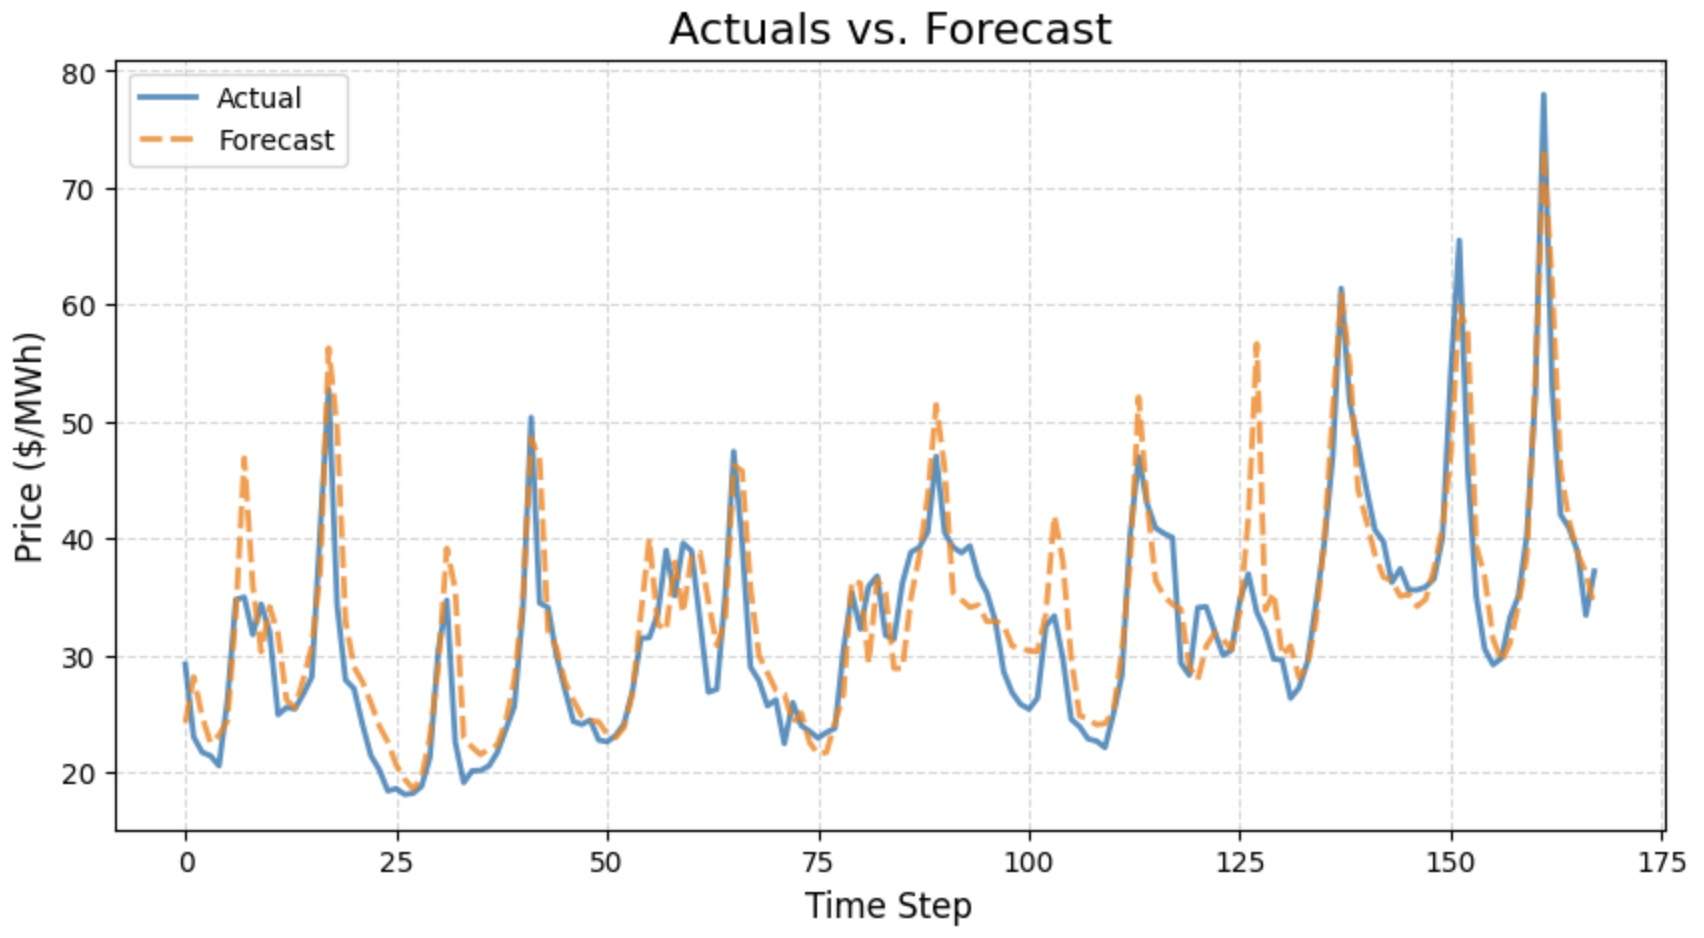
\includegraphics[width=0.8\columnwidth]{Figures/LSTM_24_1_Results.png}
\end{figure}

\subsection*{24 hours prior to predict 24 hours ahead}

\noindent Figure 19 shows the loss curve.
\begin{figure}[H]
	\centering
	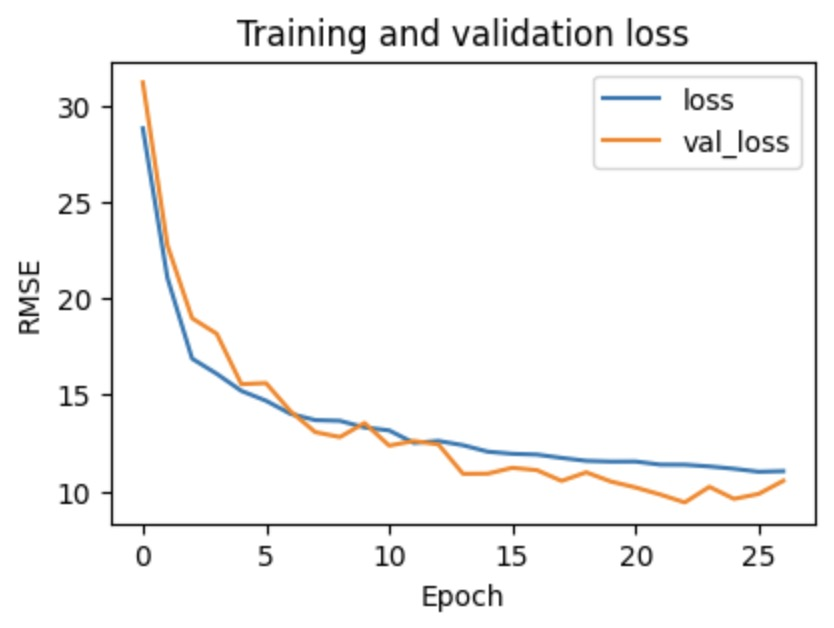
\includegraphics[width=0.8\columnwidth]{Figures/LSTM_24_24_Learning.png}
\end{figure}

\noindent Over the test dataset, an average MAPE of \textbf{23.17\%}.\\

\noindent Figure 20 shows the forecasting results for 1 week.
\begin{figure}[H]
	\centering
	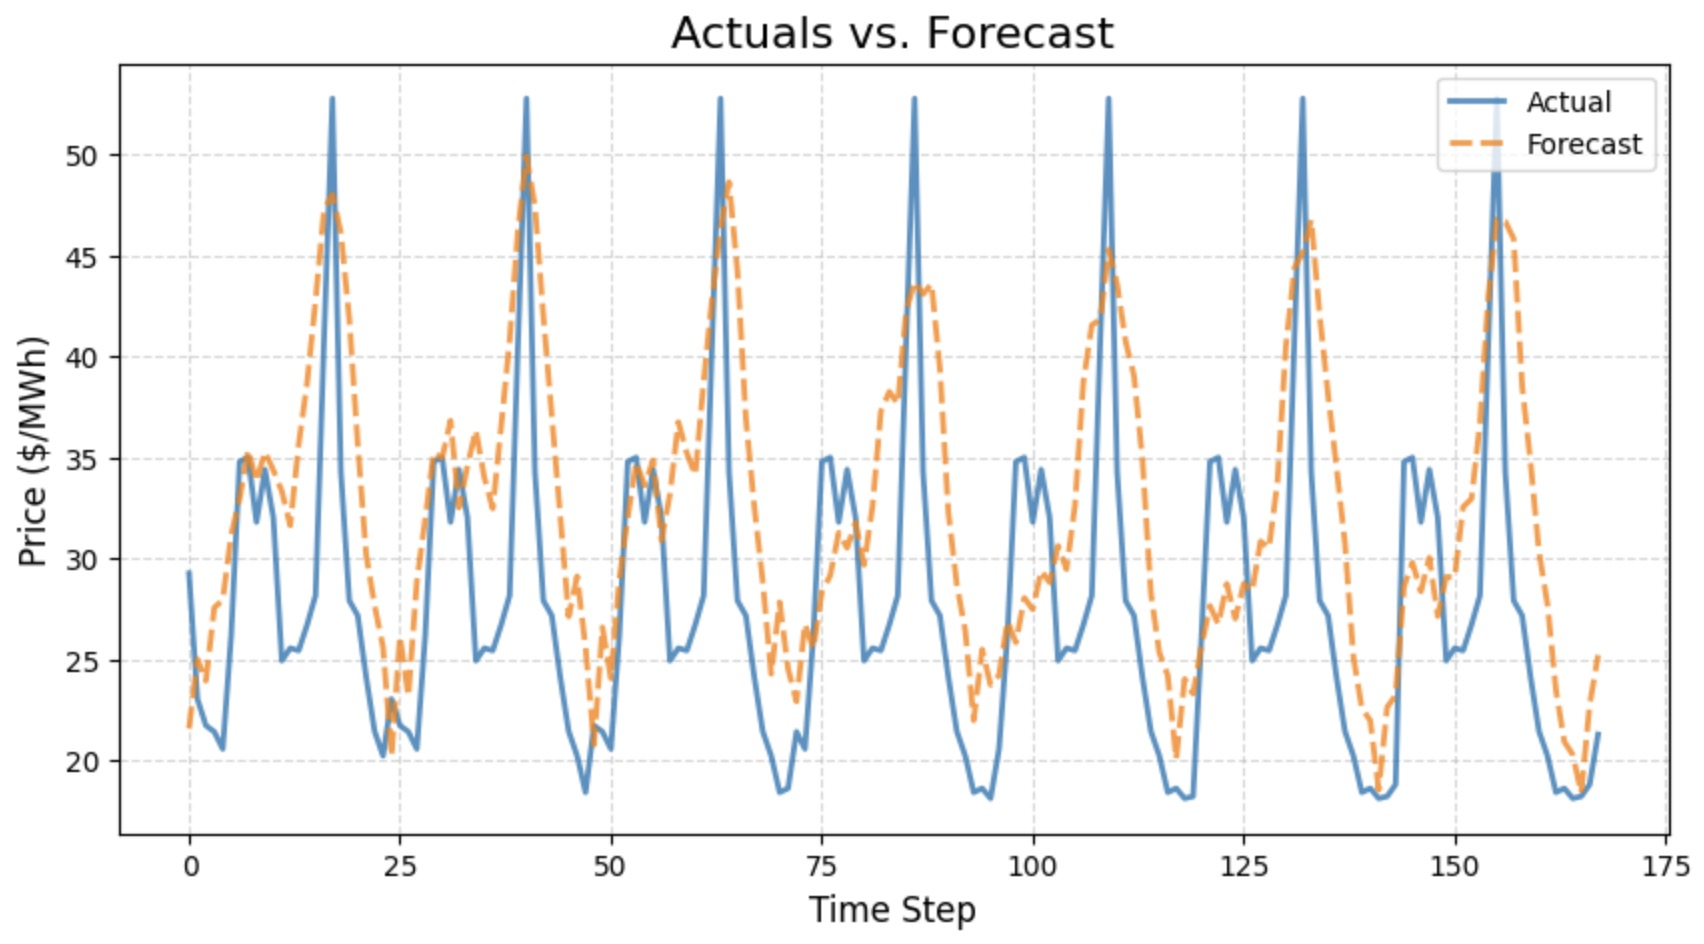
\includegraphics[width=0.8\columnwidth]{Figures/LSTM_24_24_Results.png}
\end{figure}

\noindent The results of the LSTM model do not learn well for the 24 hour-ahead model. It seems to capture the daily peaks, but not the troughs. It's strange that it wouldn't perform as well as at least the dense model. Still performed similar to the previous two models though.

\section*{CNN-LSTM ARCHITECTURE}

The proposed method in this report is a combination of convolutional layers and LSTM layers. The idea is that the convolutional layers would learn the relationships between the independent variables and then feed the output of those 1-d convolutional layers into LSTM layers to learn from the sequence of the data.

\noindent Figure 21 shows the architecture of the CNN-LSTM model.
\begin{figure}[H]
	\centering
	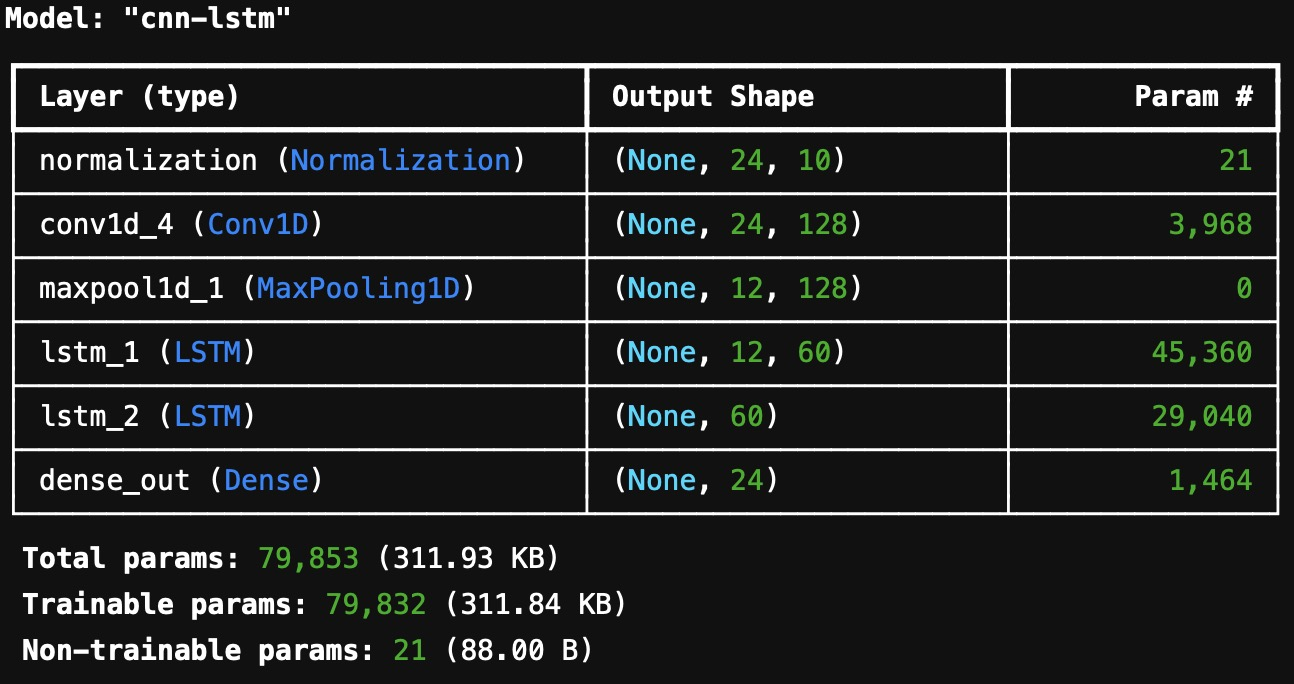
\includegraphics[width=0.8\columnwidth]{Figures/CNN-LSTM_Architecture.png}
\end{figure}

\noindent Hyperparameters:
\begin{itemize}
	\item Activation: ReLU
	\item LSTM cell units: 60
	\item Epochs: 100 /w EarlyStopping (patience=4)
	\item Optimizer: RMSProp
	\item Loss Function: RMSE
	\item Bach Size: 168
\end{itemize}


\subsection*{24 hours prior to predict 1 hour ahead}

\noindent Figure 22 shows the loss curve.
\begin{figure}[H]
	\centering
	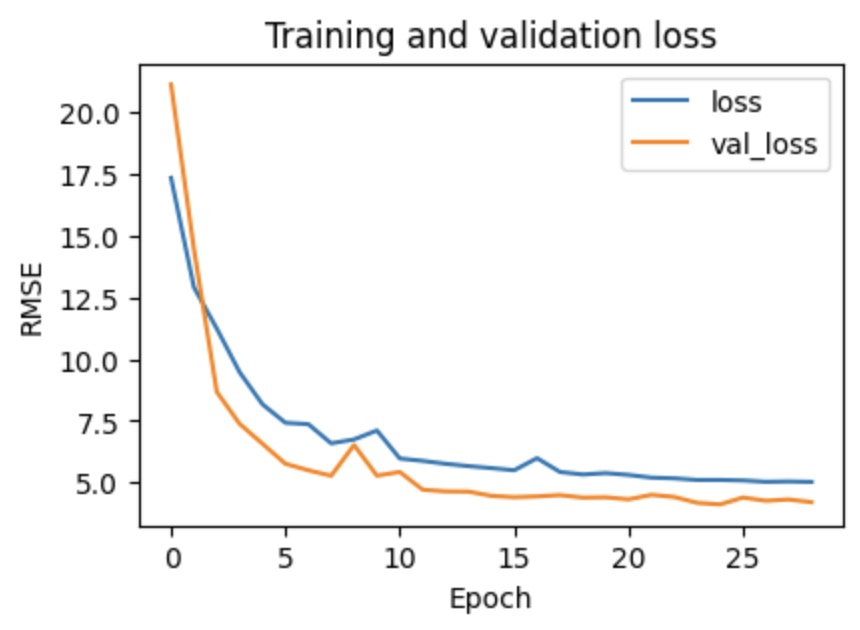
\includegraphics[width=0.8\columnwidth]{Figures/CNN-LSTM_24_1_Learning.png}
\end{figure}

\noindent Over the test dataset, an average MAPE of \textbf{9.23\%}.\\

\noindent Figure 23 shows the forecasting results for 1 week.
\begin{figure}[H]
	\centering
	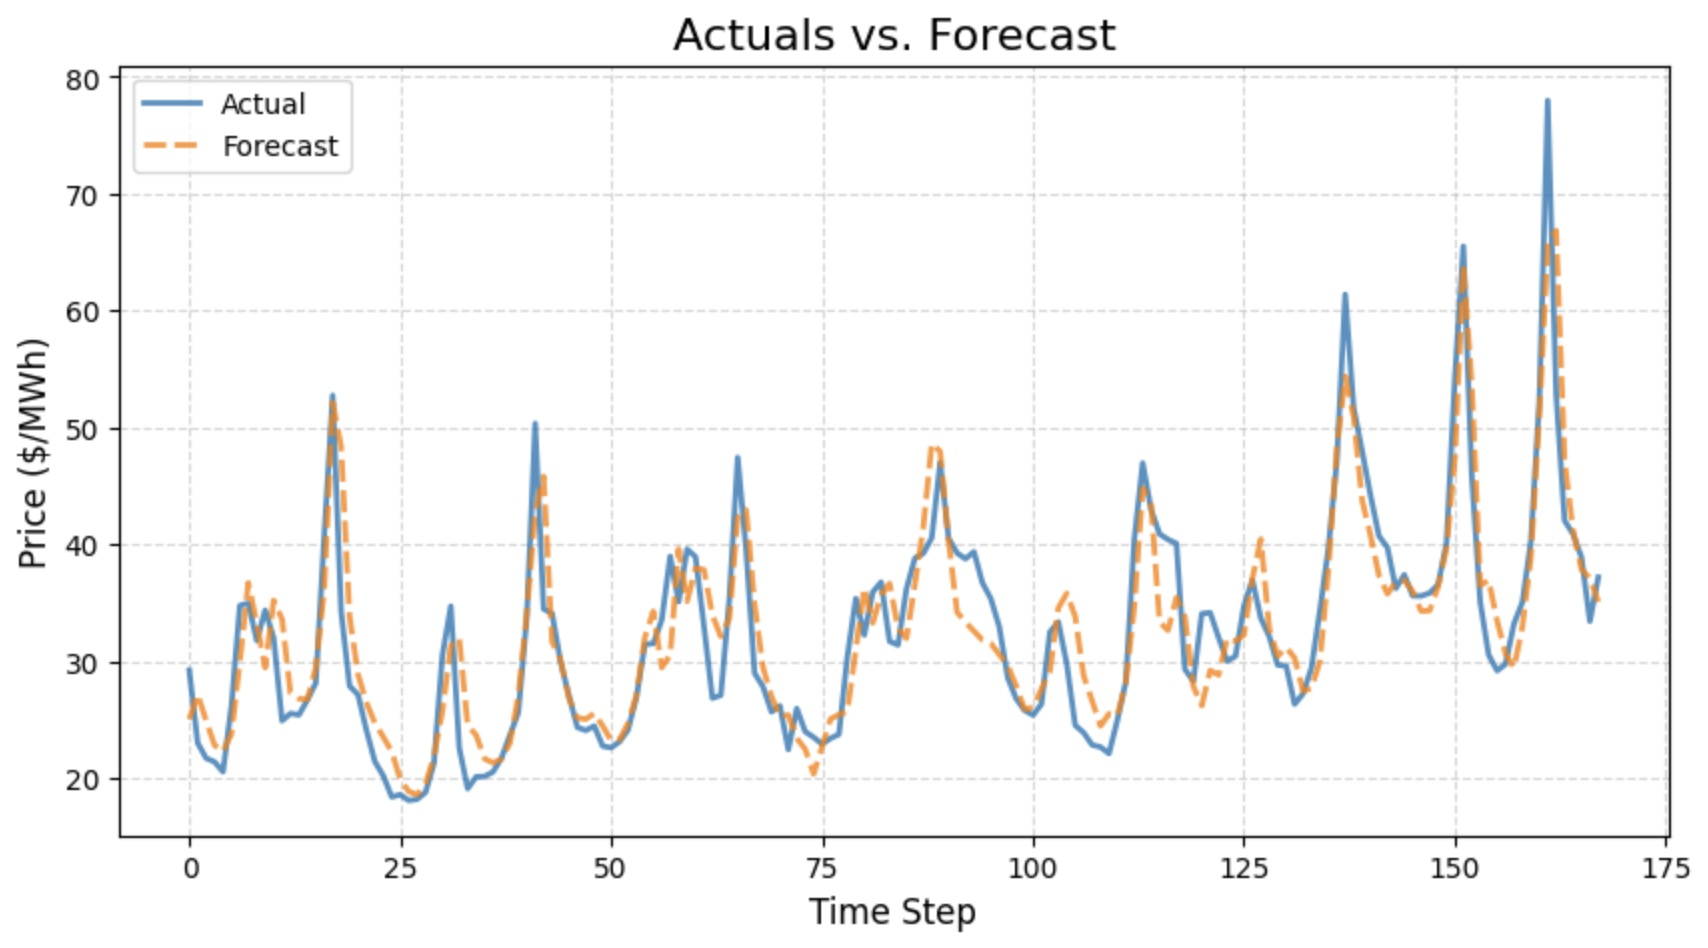
\includegraphics[width=0.8\columnwidth]{Figures/CNN-LSTM_24_1_Results.png}
\end{figure}

\subsection*{24 hours prior to predict 24 hours ahead}


\noindent Figure 24 shows the loss curve.
\begin{figure}[H]
	\centering
	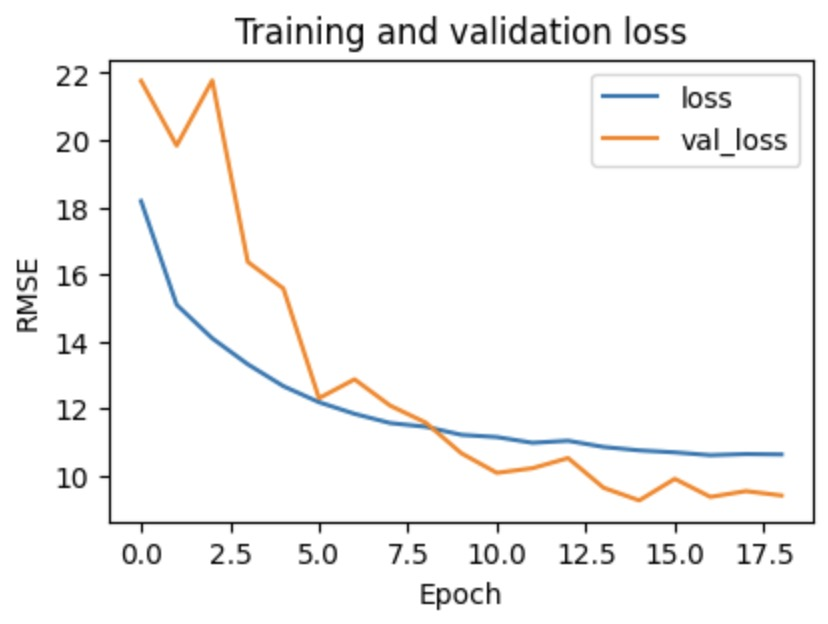
\includegraphics[width=0.8\columnwidth]{Figures/CNN-LSTM_24_24_Learning.png}
\end{figure}

\noindent Over the test dataset, an average MAPE of \textbf{21.07\%}.\\

\noindent Figure 25 shows the forecasting results for 1 week.
\begin{figure}[H]
	\centering
	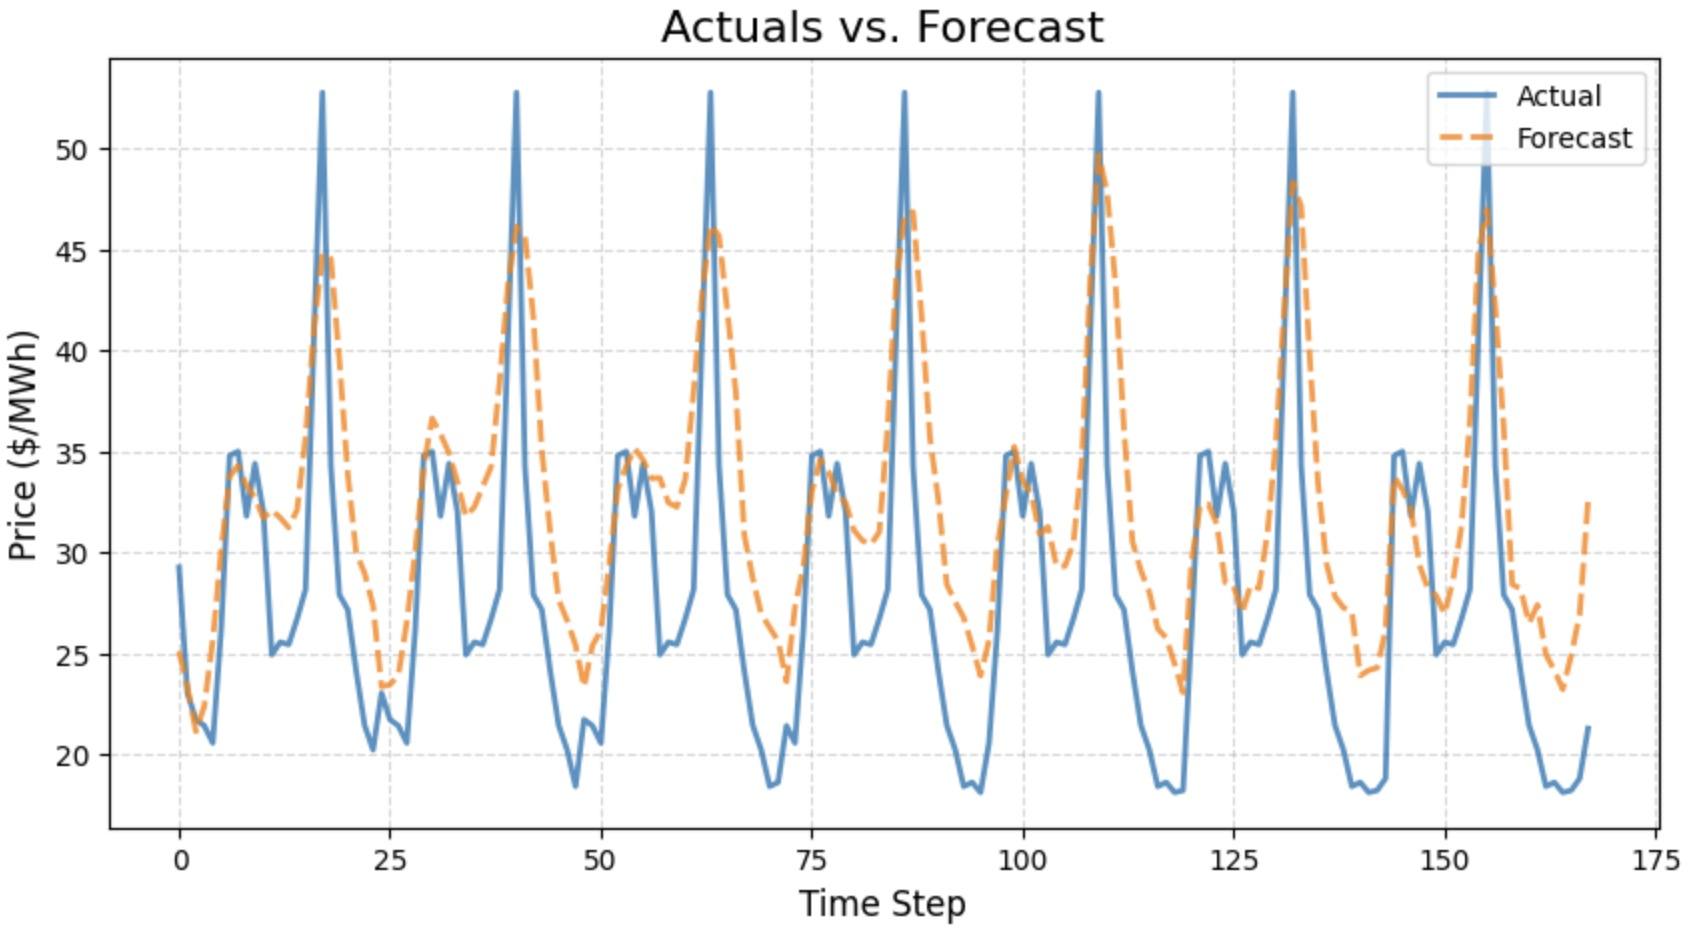
\includegraphics[width=0.8\columnwidth]{Figures/CNN-LSTM_24_24_Results.png}
\end{figure}

\section*{HYPER-PARAMETER OPTIMIZATION}

The models' hyperparameters were mostly tuned by hand. The number of epochs, batch size, number of neurons, number of units per layer, optimizer, and loss function were all adjusted carefully to get the best results given the lack of data. 

\subsection*{Genetic Algorithm}
Rather than using Keras' fit method against a model and providing hyperparameters, a Genetic Algorithm (GA) was attempted to generate the model weights. The algorithm starts at an initial population (set of weights) and evolves it over generations. The fitness function is used to determine the next population. The goal is still to minimize the loss function, just in a different way.

\noindent Sample code using pyGAD for GA.
\lstinputlisting[caption=pyGAD with Keras., language=Python]{genetic-algorithm.py}

\section*{ALL RESULTS TABLE}

Table 1, shows results for the 24 hour prior, 1 hour ahead models. 

	\begin{tabular}{lllp{12.2cm}}
		\toprule
		\textbf{Model} & \textbf{Val RMSE} & \textbf{Test MAPE} \\                                            
		\midrule
		Dense & 5.9 & 9.78\% \\
		CNN & 5.4 & 11.13\% \\
		LSTM & 5.7 & 10.66\% \\
		CNN-LSTM & 4.8 & 9.23\% \\
		\bottomrule
	\end{tabular}\\
	
\noindent Table 2, shows results for the 24 hour prior, 24 hours ahead models. 

	\begin{tabular}{lllp{12.2cm}}
		\toprule
		\textbf{Model} & \textbf{Val RMSE} & \textbf{Test MAPE} \\                                            
		\midrule
		Dense & 12.5 & 22.23\% \\
		CNN & 10.8 & 22.88\% \\
		LSTM & 11.2 & 23.17\% \\
		CNN-LSTM & 9.8 & 21.07\% \\
		\bottomrule
	\end{tabular}\\
	

\noindent These models performed decently well. It seems like the combination of CNN-LSTM has potential in the realm of day-ahead price forecasting.

\section*{FEEDBACK RESPONSE}
The main feedback for this project was that there needed to be more experimentation. I believe that I could have gotten the model better given more time, but given what I had, I think it turned out okay. One aspect that was added after the initial plan was the experimentation with GA. It didn't quite work as well as I had hoped, but it was still a great learning experience.

\section*{CONCLUSION}

Overall, I would say this project taught me many different concepts when it comes to time-series forecasting. Concepts such as stationary vs. non-stationary, windowing techniques, and different techniques for forecasting a time-series problem. For the 24 hours ahead CNN-LSTM model, I achieved a MAPE of 21\%. My goal was 15\%, but I am still happy with the results. This is a very hard problem with not many resources online about it. It's a problem that many academic journals have been written about, but in practice, it is still a very difficult problem that even energy utilities and other market participants struggle with. I hope to improve upon the CNN-LSTM architecture and incorporate more data to further improve the results. 

Uncomment the command \verb|\tableofcontents| to display it.

Remember that numberless sections will not appear in the ToC, however, you can place them manually with the command \verb|\addcontentsline{toc}{section}{section name}|.

\section*{REFERENCES}
	%----------------------------------------------------------
	
Y. Zhu, R. Dai, G. Liu, Z. Wang and S. Lu, "Power Market Price
Forecasting via Deep Learning,"
IECON 2018 - 44th Annual
Conference of the IEEE Industrial Electronics Society, Washington,
DC, USA, 2018, pp. 4935-4939, doi: 10.1109/IECON.2018.8591581.\\

\noindent Y. -Y. Hong, J. V. Taylar and A. C. Fajardo, "Locational Marginal Price
Forecasting Using Deep Learning Network Optimized by Mapping-
Based Genetic Algorithm," in
IEEE Access, vol. 8, pp. 91975-91988,
2020, doi: 10.1109/ACCESS.2020.2994444.\\

\noindent Zhang, C., Li, R., Shi, H. and Li, F. (2020), Deep learning for day-
ahead electricity price forecasting. IET Smart Grid, 3: 462-
469. https://doi.org/10.1049/iet-stg.2019.0258

	
\end{document}
© C. Albert Thompson 2016 | This page was made possible by CMH and latexindent.pl